\chapter{Interligação de componentes}
\label{interlapd}

\begin{figure}[h]
	\centering
	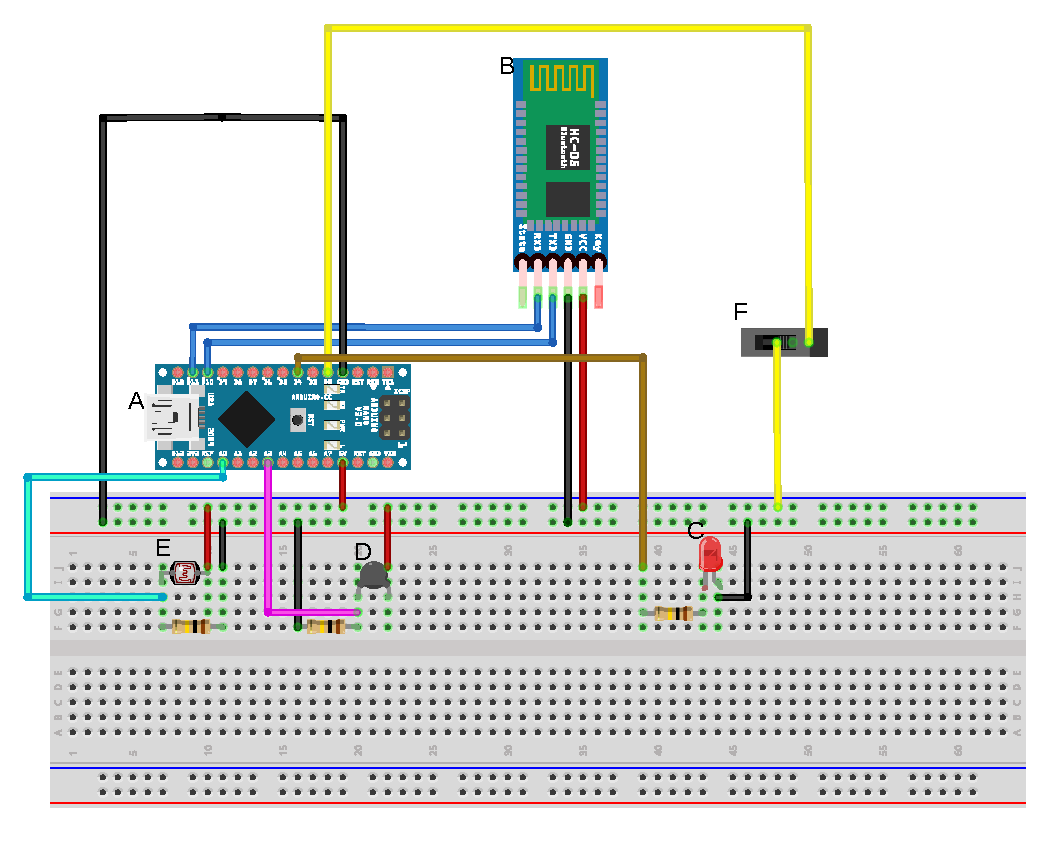
\includegraphics[width=\linewidth]{esquemas/arduino-fritzing/esquema-arduino_bb.pdf}
	\caption{Protótipo da solução em \textit{hardware} desenvolvida}
	\label{hardwaProt}
\end{figure}

Na figura \ref{hardwaProt} encontra-se o esquema da interligação dos diferentes componentes de \textit{hardware} numa placa de prototipagem (placa branca). 


\textbf{Legenda: }

\begin{itemize}
	\item \textbf{A}: Arduino Nano
	\item \textbf{B}: Módulo Bluetooth HC-06
	\item \textbf{C}: \ac{LED}
	\item \textbf{D}: Sensor de temperatura TTC 104 NTC
	\item \textbf{E}: Sensor de luminosidade GL5528 (foto-resistência) 
	\item \textbf{F}: Sensor para nível de água 
\end{itemize}